\section{Carnot-Prozess}
\begin{figure}[H]
  \centering
  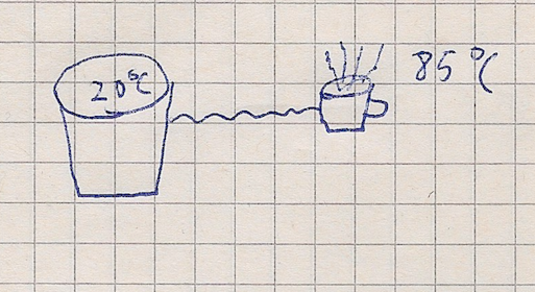
\includegraphics[width = \textwidth]{Zeichnungen/18.pdf}
  \caption{Zwei Systeme mit unterschiedlicher Temperatur.}
  %\label{fig:Bild}
\end{figure}
\paragraph{Kelvin:} Es gibt keinen zyklischen thermodynamischen Prozess, dessen einziger Effekt ist, einem Wärmereservoir Wärme zu entziehen  und diese völlig in Arbeit zu verwandeln.

% \begin{figure}[H]
%   \centering
%   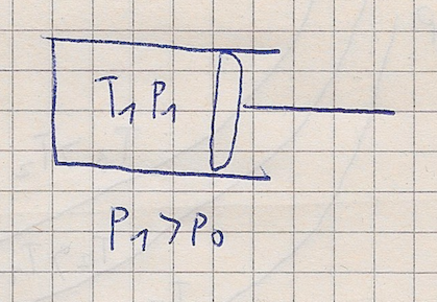
\includegraphics[width = \textwidth]{Zeichnungen/19.pdf}
%   \caption{Kolben.}
%   %\label{fig:Bild}
% \end{figure}
\begin{figure}
\centering
\begin{tikzpicture}
            \draw (0,1) rectangle (3, 2.5)
             (2,1) rectangle (2.5, 2.5)
             (2.5, 1.7) rectangle (6, 1.8)
             (1,1.75) node {$T V P_1$}
             (1, 0) node {$P_1 > P_0$};
\end{tikzpicture}
\caption{Kolben}
\end{figure}
\paragraph{Clausius:} Es gibt keinen zyklischen thermodynamischen Prozess, dessen einziger Effekt es ist Wärme von einem kalten Reservoir in ein wärmeres zu bringen. (Perpetuum Mobile 2. Art)  
\begin{itemize}
    \item Clausius $\Rightarrow$ Kelvin
    \item Wenn Kelvin falsch $\Rightarrow$ Clausius falsch
    \item entziehe Reservoir Wärme $\Rightarrow$ Arbeit
    
\end{itemize}
\paragraph{Carnotprozess}
\begin{figure}[H]
  \centering
  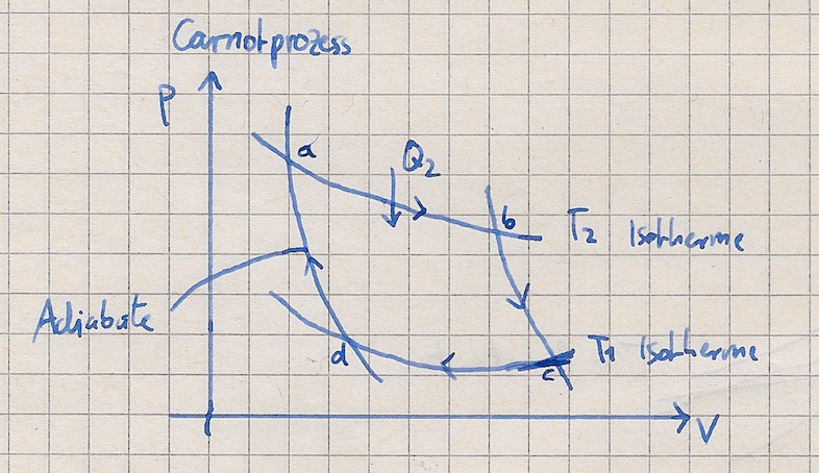
\includegraphics[width = \textwidth]{Zeichnungen/20.pdf}
  \caption{Der Carnotprozess.}
  %\label{fig:Bild}
\end{figure}
\begin{figure}[H]
  \centering
  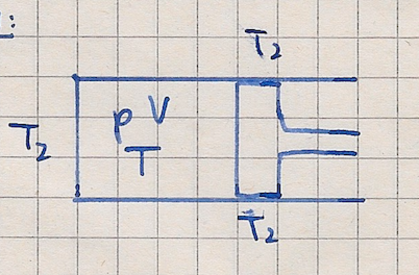
\includegraphics[width = \textwidth]{Zeichnungen/21.pdf}
  \caption{Kolben mit Temperaturangabe.}
  %\label{fig:Bild}
\end{figure}
\begin{figure}[H]
  \centering
  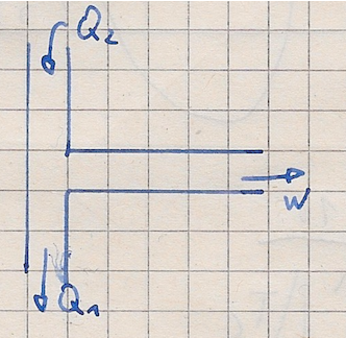
\includegraphics[width = \textwidth]{Zeichnungen/22.pdf}
  \caption{System mit Wärmeaufnahme und -abgabe und Arbeitabgabe.}
  %\label{fig:Bild}
\end{figure}
\begin{figure}
\centering
\begin{tikzpicture}
            \draw (0,0) rectangle (3,1.5)
             (2,0) rectangle (2.5, 1.5)
             (2.5, 0.7) rectangle (6, 0.8)
             (1,0.75) node {$P\ V\ T$}
             (1, -0.5) node {$T_2$}
             (-0.5, 0.75) node {$T_2$}
             (1, 2) node {$T_2$};
\end{tikzpicture}
\end{figure}

\begin{figure}
\centering
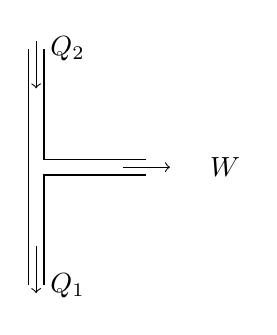
\begin{tikzpicture}
            \draw (0,0) -- (0,3)
                  (0.2, 0) -- (0.2, 1.4) -- (1.5,1.4)
                  (1.5, 1.6) -- (0.2, 1.6) -- (0.2, 3)
                  [->] (0.1, 0.5) -- (0.1, -0.1);
            \draw [->] (0.1, 3.1) -- (0.1, 2.5);
            \draw [->] (1.2, 1.5) -- (1.8, 1.5);
            \draw (0.5, 0) node {$Q_1$}
                  (0.5, 3) node {$Q_2$}
                  (2.5, 1.5) node {$W$};
\end{tikzpicture}
\end{figure}

\begin{align}
    \frac{pV}{T} &= N k_B\\
    P &= \frac{N k_\text{B} T}{V}
\intertext{Adiabaten immer steiler als Isotherme}
    \dif U &= \delta Q - \delta W\\
    &= T\dif S - p \dif V\\
    U &= \frac32 k_\text{B} N T\\
    \dif U&=0  \\
    \delta U &= T \dif S \\
    Q &= T_2 (S_b-S_a)\\
\intertext{Verrichtete Arbeit}
    \int p \dif V&= N k_B T_2 \int_a^b \frac{\dif V}{V}\\
    &= N k_B T \ln\left(\frac{V_b}{V_a}\right)\\
    (S_b - S_a) &= k_\text{B} N \ln \left(\frac{V_b}{V_a}\right)\\
\intertext{Adiabatische Expansion}
    \delta Q &= 0\\
    \dif U &= -p \dif V \\
    \Delta U &= \frac32 k_B N (T_2-T_1)\\
    \dif U &= \frac 3{2} k_\text{B} N \dif T = -p \dif V = -\frac{N k_\text{B} T}{V} \dif V\\
    \int_b^c \frac{\dif V}{V}&=-\frac 32 \frac{\dif T}{T}\\ 
    \ln\left(\frac{V^c}{V_b}\right) &= \ln\left(\frac{T^c}{T_b}\right)^{-3/2}\\
    V &= V_b \left(\frac{T}{T_b}\right)^{-3/2}\\
    V T^{\frac{3}{2}} &= \frac{V_b}{T_b^{-\frac 32}}= \text{const.} 
\intertext{Adiabatengleichung für ideales Gas}
    V^{\frac{2}{3}} T &= \text{const.} \\
    T V^{\varkappa-1} &= \text{const.}  \quad \varkappa = \frac{C_p}{C_V} = \frac{C_V+R}{C_V} = \frac{\frac{5}{2}}{\frac{3}{2}}\\
\intertext{ideales Gas}
    C_V&=\frac 32 R\\
    C_p-C_V&=R\\
    \varkappa&= \frac{5}{3}\\
    \Aboxed{ \varkappa -1 &= \frac{2}{3}}\\
    \Aboxed{\dif U &=0 \quad \text{Gesamtprozess}}
\end{align}
\begin{figure}[H]
  \centering
  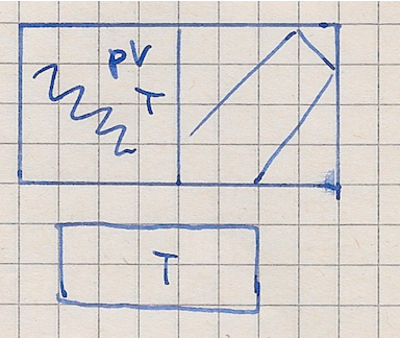
\includegraphics[width = \textwidth]{Zeichnungen/23.pdf}
  \caption{Zwei Systeme.}
  %\label{fig:Bild}
\end{figure}
\begin{align}
    \text{Wirkungsgrad} \quad  \eta &= \frac{\text{geleistete Arbeit}}{\text{aufgenommene Wärme}}\\
    \eta &= \frac{Q_2 - Q_1}{Q_2} = 1- \frac{Q_1}{Q_2} \quad Q_1 = 0 \Rightarrow \text{bestmöglicher Prozess}
\end{align}
Zeige, dass dies so ist (Huang)
\begin{enumerate}
    \item Maschine X
    \item Carnotprozess C
    \item $\Rightarrow$ Beide zwischen $T_1$ und $T_2$
\end{enumerate}
\begin{figure}[H]
  \centering
  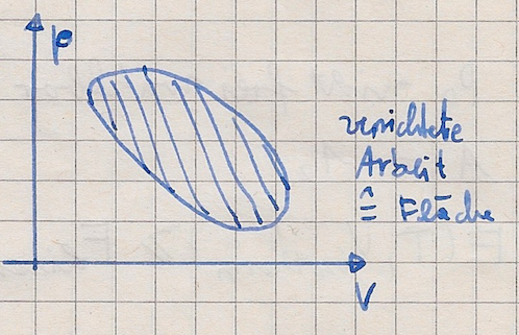
\includegraphics[width = \textwidth]{Zeichnungen/24.pdf}
  \caption{Verrichtete Arbeit in einem Kreisprozess.}
  %\label{fig:Bild}
\end{figure}
\begin{align}
    X \to W' \\
    C \to W  \\
    W_\text{total} &= N'W' - N W \\
    Q_\text{2, total} &= N' Q_2' - N Q_2 = 0\\
    Q_\text{1, total} &= N' Q_1' - N Q_1\\
    W_\text{total} &= N' W' - N W = \cancel{Q_\text{2, total}} - Q_\text{1, total} = - Q_\text{1,total} \\
    \underarrow{W_\text{total} > 0 }{\text{Widerspruch zu Kelvin}}\\
    \Aboxed{\Rightarrow W_\text{total}} \leq 0 \quad \text{\enquote{Unten wird Wärme abgegeben}}
\end{align}

\begin{align}
    N'&=\frac{Q_2}{Q_2'}  N\\
    Q_\text{1 total}&= N' Q_1' -N_1 Q_1 \geq 0\\
    \frac{Q_2}{Q_2'} N Q_1'-N_1 Q_1 &\geq 0 \quad \bigg \rvert \quad \frac{Q_2'}{N} \\
    Q_2 Q_1' &\geq Q_2' Q_1\\
    \frac{Q_1}{Q_2} &\geq \frac{Q_1'}{Q_2'}\\
    \Aboxed{1-\frac{Q_1}{Q_2} &\geq 1- \frac{Q_1'}{Q_2'}}\\
    \eta_c &\geq \eta_x 
\end{align}
\begin{figure}[H]
  \centering
  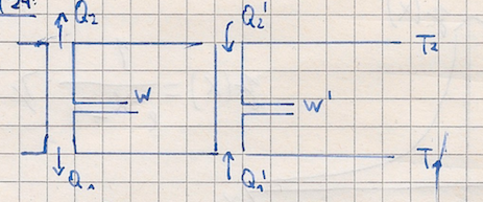
\includegraphics[width = \textwidth]{Zeichnungen/24b.pdf}
  \caption{???.}
  %\label{fig:Bild}
\end{figure}

Alle Carnotmaschinen die zwischen $T_1$ und $T_2$ \enquote{laufen} haben den gleichen Wirkungsgrad. Unabhängig von Arbeitsstoff und Konstruktion.
Möglichkeit die Temperatur materialunabhängig zu definieren.
\begin{align}
    \frac{Q_2}{Q_1}&=f(T_1,T_2)   & \frac{Q_2}{Q_1}&=\frac{\theta(T_2)}{\theta (T_1)} \\
    \delta Q &= C_V \dif T + \delta W & C_V &= \pdif{U}{T} \\
    \dif S &= \frac{\delta Q}{T}=C_V \frac{\dif T}{T} +\frac{R \dif V}{V} \\
 \text{(vollständiges Differential)}
  \end{align}

\begin{figure}[H]
  \centering
  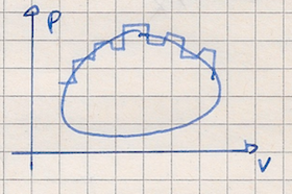
\includegraphics[width = \textwidth]{Zeichnungen/25.pdf}
  \caption{Mögliche Stufenform im p-V-Diagramm.}
  %\label{fig:Bild}
\end{figure}
\begin{align}
    S(T,V)&=C_V \int_{T_0}^T \frac{\dif T_0}{T} + R \int_{V_0}^V \frac{\dif V}{V}\\
    &= C_V \ln\left(\frac{T}{T_0}\right) + R \ln\left(\frac{V}{V_=}\right)\\ 
    &= \ln\left(\left(\frac{T}{T_0}\right)^{C_V} \left(\frac{V}{V_0}\right)^R \right)\\
    &= \ln\left( \left(\frac{T}{T_C}\right)^{C_V} \left(\frac{V}{V_0}\right)^{C_p-C_V}\right) \\
    \oint \frac{\delta Q}{T} &= 0 \quad \text{reversibel}
\end{align}